% 2  Previous Work
% 2.1  Problem setup picture(s) (which shows all variables)
% 2.2  Assumptions
% 2.3  NLSWEs ? derived from conservation of mass and Newton?s Second Law under assumptions (Just mention, not actually derive)
% 2.3.1  Mention that the SWEs have no dispersion ? there is very little dispersion near shore so this is where SWEs apply? fact check and/or more info
% 2.4  Very brief overview of how NLSWEs are linearized for arbitrary cross section
% 2.4.1  Properties of new system
% 2.4.2  Include equations to get back to physical variables
% 2.4.3  Analytical F(?) and thus W(?) for |y|^m case

	\begin{frame}
		\frametitle{Introduction to the Bay Shapes}
		In the field of Tsunami run-up research, there are several natural bay shapes to examine:
		\begin{itemize}
			\item The plane beach;
			\item Bays of parabolic cross-section;
		\end{itemize}
		There has been extensive study of the plane beach and bays of parabolic cross-section, but tsunami behavior in bays of general U-shaped bays of finite length has not been examined.
		
		In each case, we assume that the bottom profile is separable: \emph{i.e.}
		\[   z(x,y) = f(y) - h(x)  \]
		where $z(x,y)$ is the bottom profile, $f(y)$ is an arbitrary function and $h(x)$ is an arbitrary non-negative function.
	\end{frame}

	\slide[The Plane Beach]{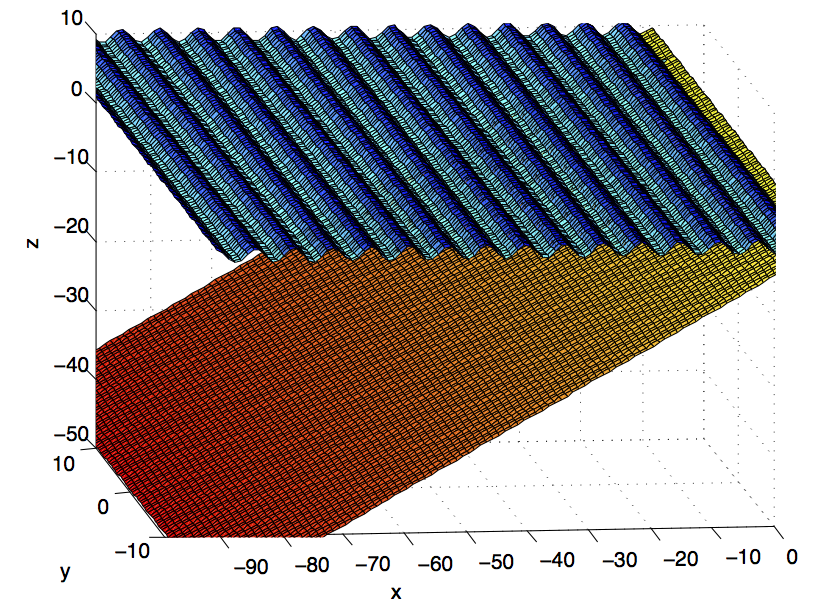
\includegraphics[width=\linewidth]{bay/planebeach.png}}

	\begin{frame}
	\frametitle{The Plane Beach}
		Characteristics of the plane beach:
		\begin{itemize}
			\item Constant slope;
			\item Uniform across y-axis;
			\item Can be simplified to 2 dimensions.
		\end{itemize}
		This is the problem examined in the famous 1958 paper of Carrier and Greenspan. They showed that in this case, explicit solutions to the shallow water wave equations were possible.
	\end{frame}

	\slide[Bays of Parabolic Cross-section]{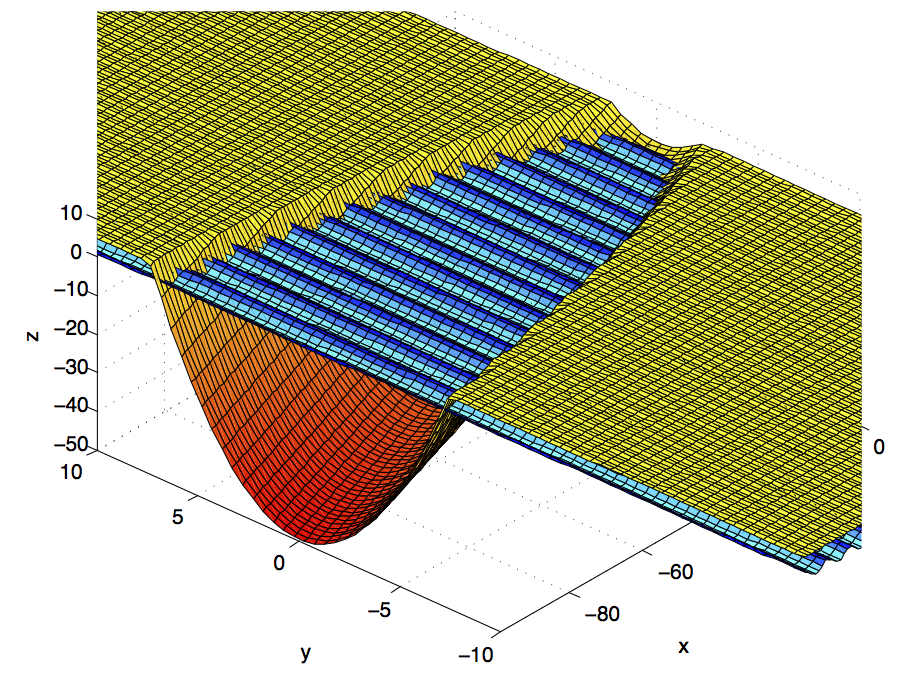
\includegraphics[width=\linewidth]{bay/parabolicbay.png}}

	\begin{frame}
		\frametitle{Bays of Parabolic Cross-section}
		Characteristics of bays of parabolic cross-section:
		Characteristics of bays of parabolic cross-section:
		\begin{itemize}
			\item Constant slope;
			\item Parabolic cross-section along y-axis;
			\item Behavior of waves in such a channel can still be simplified to 2 dimensions.
		\end{itemize}
		This more complicated problem was analyzed in a recent paper by Dr. Ira Didenkulova and Dr. Efim Pelinovsky, in which they showed that it was possible to reduce this problem to one that is analogous to the 2-dimensional case, and thus analytical solutions are possible for the infinite length case.
	\end{frame}

	

	\begin{frame}
		\frametitle{Further Terminology}
		There are a few other terms we use:
		\begin{itemize}
			\item $\eta(x,t)$ is the perturbation away from the normal water level at time $t$ and distance $x$ from shore.
			\item $H(x,t)$ is the total water depth. Note that $H(x,t) = h(x) + \eta(x,t)$.
			\item Note that for all the cases we will consider, $h(x) = -\alpha x$, where $\alpha$ is a non-negative constant. Since $x$ is typically negative in our domain, $h$ will usually be non-negative, and $H$ must always be non-negative.
		\end{itemize}
	\end{frame}

	

	\begin{frame}
		\frametitle{Wave Equation*}
		% Put the basic assumptions and talk about the general idea but do not derive everything
		% It took too much time when I gave my talks and it does not help to gain a better understanding
		% We will need the time to get through the results and explaining how the solution works
		% Ill leve it up to you to talk about eulers eq and the C of Mass eq and the assumptions/ make the slides you want.
		From this point forward, we use the symbol $u$ to represent $\bar{u}$.  Thus,
		\begin{framed} \begin{align}
			\frac{\partial S}{\partial t} + \frac{\partial}{\partial x}(uS) &= 0, \label{swe1}\\
			\frac{\partial u}{\partial t} + u \frac{\partial u}{\partial x} + g \frac{\partial H}{\partial x} &= g \frac{dh}{dx}. \label{swe2}
		\end{align} \end{framed}
		These are the wave equations that we will attempt to solve for our bays.
		% I will mention no dispersion and the compairison when you are done with your part (no slide)
	\end{frame}


\section{Mathematical Setup}

	\begin{frame}
		\frametitle{Transformation to $\sigma$, $\lambda$}
		We begin with the non-linear shallow water equations
		\begin{align} 
			\tag*{\eqref{swe1}}
			\frac{\partial S}{\partial t} + \frac{\partial}{\partial x} (uS) &= 0  \\
			\tag*{\eqref{swe2}}
			\frac{\partial u}{\partial t} + u \frac{\partial u}{\partial x} + g \frac{\partial H}{\partial x} &= g \frac{dh}{dx}
		\end{align}
		where $S$ is the cross-sectional area, $u$ is the averaged flow velocity, and $H = \eta(x,t) + h(x)$, where $h$ is unperturbed water depth and $\eta$ is the height of the perturbation.
		
		We have initial conditions that at $t=0$, $u(x,0) = 0$ and $\eta(x,0) = \eta_0(x)$, and boundary conditions that at $x=L$, $\frac{u(x_L,t)}{F(\sigma_{x_L})}=0$ 'wall' and that at the moving shoreline, $u(x,t)$ is bounded.
		
	\end{frame}


\begin{frame}
\frametitle{Riemann Invariants}
From these two equations, we can find Riemann Invariants
\[
I_\pm = u \pm \int \sqrt{\frac{g}{S}\frac{dS}{dH}} dH + g \alpha t
\]
Applying these to \eqref{swe1} and \eqref{swe2}, we get
\begin{equation}\label{invariants1}
\frac{\partial I_\pm}{\partial t} + c_{\pm} \frac{\partial I_\pm}{\partial x} = 0
\end{equation}
where
\[
c_\pm = u \pm \sqrt{g S \frac{dH}{dS}}.
\]
Note that we can write \eqref{invariants1} as
\[
\frac{\partial (I_\pm, x)}{\partial (t,x)} + c_\pm \frac{\partial(t, I_\pm)}{\partial (t,x)} = 0.
\]
\end{frame}

\begin{frame}
\frametitle{Hodograph Transform}
We apply a hodograph transform with Jacobian $\dfrac{\partial (t,x)}{\partial(I_+, I_-)}$. This Jacobian will be zero if, and only if, the wave breaks before it reaches shore. After applying the transform, we see that
\[
\frac{\partial(I_\pm,x)}{\partial(I_+,I_-)} + c_\pm \frac{\partial (t, I_\pm)}{\partial(I_+,I_-)} = 0,
\]
which can be written as
\begin{equation}\label{hodograph}
\frac{\partial x}{\partial I_\pm} - c_\mp \frac{\partial t}{\partial I_\pm} = 0.
\end{equation}
\end{frame}

\begin{frame}
\frametitle{Change of Variables}
We define two new variables:
\[
\lambda = \frac{I_+ + I_-}{2} \text{ and } \sigma = \frac{I_+ - I_-}{2}.
\]
Notice that this implies that
\begin{equation} \label{siglam}
\lambda = u + \alpha g t \text{ and } \sigma = \int_0^H \sqrt{\frac{g}{S} \frac{dS}{dH}}dH.
\end{equation}
We also define
\[
F(\sigma) = c_+ - c_- = 2 \sqrt{gS \frac{dH}{dS}}.
\]
\end{frame}

\begin{frame}
\frametitle{Change of Variables 2}
In these new variables, \eqref{hodograph} becomes
\[
\frac{\partial^2 t}{\partial \lambda^2} - \frac{\partial^2 t}{\partial \sigma^2} - \left( \frac{2 + \frac{dF}{d\sigma}}{F(\sigma)} \right) \frac{\partial t}{\partial \sigma} = 0,
\]
which, because of how $u,t,$ and $\lambda$ are related in \eqref{siglam}, is equivalent to
\begin{equation}\label{finalu}
\frac{\partial^2 u}{\partial \lambda^2} - \frac{\partial^2 u}{\partial \sigma^2} - \left( \frac{2 + \frac{dF}{d\sigma}}{F(\sigma)} \right) \frac{\partial u}{\partial \sigma} = 0.
\end{equation}
So we can find $t$ and $u$.
\end{frame}

\begin{frame}
\frametitle{Finding a relation for $x$}
In order to find $x$, we also obtain from \eqref{hodograph} that
\[
g \alpha \frac{\partial x}{\partial \sigma} = - u \frac{\partial u}{\partial \sigma} - \frac{F(\sigma)}{2} + \frac{F(\sigma)}{2} \frac{\partial u}{\partial \lambda}.
\]
To integrate this, we define a potential function $\Phi(\sigma,\lambda)$ by
\[
u = \frac{1}{F(\sigma)} \frac{\partial \Phi}{\partial \sigma}.
\]
Then we see that
\[
2 g \alpha x = \frac{\partial \Phi}{\partial \lambda} - \int_0^\sigma F(\sigma) d\sigma - u^2 = \frac{\partial \Phi}{\partial \lambda} - 2gH - u^2.
\]
Hence
\[
\eta = H - h = H + \alpha x = \frac{1}{2g} \left(\frac{\partial \Phi}{\partial \lambda} - u^2 \right)
\]
\end{frame}








\begin{frame}
\frametitle{Backsubstituting to Physical Variables}
We have the following backsubstitution equations:
\[
u = \frac{\phi_\sigma}{F(\sigma)} \text{ and } \eta = \frac{1}{2g}\left(\phi_\lambda - u^2\right)
\]
\[
x = \frac{1}{2g\alpha} \left(\phi_\lambda - 2gH - u^2 \right) \text{ and } t = \frac{\lambda - u}{\alpha g}.
\]
We know that this backsubstitution is possible because the 4-part Jacobian matrix
\[
\frac{\partial (x,t,u,\eta)}{\partial (\sigma,\lambda,\phi_\sigma,\phi_\lambda)}
\]
has a non-zero determinant.
\end{frame}


\begin{frame}
\frametitle{Writing an Equation in Terms of $\Phi$}
We substitute our definition of $\Phi$ into \eqref{finalu} to obtain
\begin{equation}\label{Phieq}
\frac{\partial^2 \Phi}{\partial \lambda^2} - \frac{\partial^2 \Phi}{\partial \sigma^2} - W(\sigma) \frac{\partial \Phi}{\partial \sigma} = 0,
\end{equation}
where
\[
W(\sigma) = \frac{2 + \frac{dF}{d\sigma}}{F(\sigma)}.
\]
We can think of $\sigma$ as a space-like variable and $\lambda$ as a time-like variable. So we have initial conditions at $\lambda = 0$,
\end{frame}


\begin{frame}
\frametitle{Finding $F$ and $W$ for U-shaped bays}
We need to find $F(\sigma)$ for the case of a U-shaped bay ($|y^m|$). Recalling that
\[
F(\sigma)= 2 \sqrt{gS \frac{dH}{dS}} \text{ and } \sigma = \int_0^H \sqrt{\frac{g}{S} \frac{dS}{dH}}dH.
\]
By integrating we can write $S(H)=2\frac{m}{m+1}H^{\frac{m+1}{m}}$ and also
\[
F(H)=2\sqrt{g} \sqrt{\frac{m}{m+1}} \sqrt{H} \text{ and } \sigma=2\sqrt{\frac{g(m+1)}{m}} H^{\frac12}
\]
So
\[F(\sigma)=\frac{m}{(m+1)\sigma}
\]
and
\[
W(\sigma) = \frac{2 + \frac{dF}{d\sigma}}{F(\sigma)}=\frac{m+2}{m\sigma}.
\]

\end{frame}




